\documentclass{article}

% set font encoding for PDFLaTeX or XeLaTeX
\usepackage{ifxetex}
\ifxetex
  \usepackage{fontspec}
\else
  \usepackage[T1]{fontenc}
  \usepackage[utf8]{inputenc}
  \usepackage{lmodern}
  \usepackage{float}
  \usepackage{graphicx}
  \usepackage{morefloats}
  \usepackage{wrapfig}
\fi


% used in maketitle
\title{Actividad 3}
\author{Fátima Brambilla}
\date{14 de Febrero, 2018}
% Enable SageTeX to run SageMath code right inside this LaTeX file.
% documentation: http://mirrors.ctan.org/macros/latex/contrib/sagetex/sagetexpackage.pdf
% \usepackage{sagetex}

\begin{document}
\maketitle

\section {Introducción}
En la tercera actividad continuamos practicando la utilización del entorno de programación de \textit{Python}, así como el uso de las bibliotecas \textit{Pandas}, \textit{Matplotlib}, apoyándonos en el entorno de programación de \textit{Jupyter Notebook}.
Para esta actividad nos apoyamos en los datos de sondeos atmósfericos de la pagina de la \textit{Universidad de Wyoming}. Como en la actividad anterior, prácticamos la creación de gráficas con datos obtenidos de una pagina web oficial.

\section {Fundamentos}
Los fundamentos de esta práctica están en el conocimiento de las herramientas que necesitaríamos. Entre ellas, las bibliotecas \textit{Pandas}, y \textit{Matplotlib}, la primera es una librería de linsencía libre,que provee un alto rendimiento, y  una forma sencilla de utilizar la estructura de datos, y las herramientas de ánalisis para el lenguaje de programación de Python. La segunda, matplotlib es una librería de trazado en 2D, la cual produce gráficas de alta calidad para la publicación. Esta librería puede ser utilizada en diferentes pythons, en jupyter notebook, en aplicaciones web, entre otros.
Otras cuestiones que debían estar claras antes de empezar a trabajar, eran las capas de la atmósfera, sin embargo, esto lo estudiamos durante la primera actividad, de forma que solo mencionaremos sus nombres
\begin{enumerate}
\item Trotósfera
\item Estratósfera
\item Mesósfera
\item Termósfera
\item Exósfera
\end{enumerate}
Cabe mencionar que, los datos recaudados de la pagina de la universidad de Wyoming,son datos de fénomenos meteorológicos, las cuales ocurren entre las capas atmósfericas previamente mencionadas.

\section{Procedimiento y Ánalisis de Datos}
Lo primero fue obtener los datos de una estación de servicio, de dos días del año 2017, el 22 de Junio, y el 22 de Diciembre, de forma que pudierámos hacer una comparación de ambos días por medio de gráficas en base a los datos recogidos.
Al tener los datos, se abrieron ambos archivos en emacs, para ser editados a conveniencia antes de empezar a trabajar en python con ellos. Una vez que fueron editados, se empezó a trabajar en Jupyter Notebook, asignando una etiqueta a cada archivo para la comodidad al momento de trabajar.
Se le pidió al programa que analizará ambos archivos, para después empezar a trabajar con distintas gráficas que nos eran solicitadas en la actividad, cada tipo de gráfica para ambos archivos. La primera era una gráfica que mostraba el cambió en la presión atmósferica con respecto a la altura. Se nos dio un ejemplo de como debía lucir esa tabla.
Las siguientes tablas eran sobre la temperatura y la temperatura del roció, ambas puestas en función de la altura, en esta gráfica, se comparan ambas "variables" en un solo gráfico. La siguiente era un gráfico que mostraba la velocidad de los vientos en nudos, y por último se hizo una gráfica de la húmedad relativa en función de la altura

\section{Resultados}
Las siguientes dos gráficas son las primeras que se hicieron, son las que mostraban el cambio en la presión en función de la altura.
\begin{figure}[H]
    \caption{Variación de la Presión en Función de la Altura(Diciembre)}
    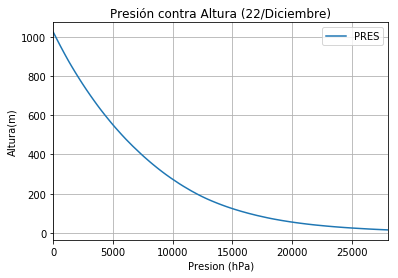
\includegraphics[width=0.5\textwidth]{VarPresion-AlturaDic.png}
    \centering
    \label{Pre-Alt}
\end{figure}

\begin{figure}[H]
    \caption{Variación de la Presión en Función de la Altura(Junio)}
    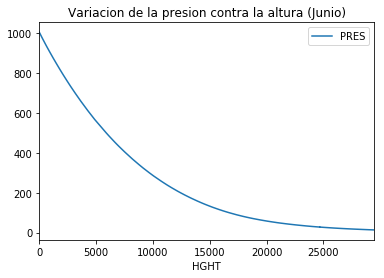
\includegraphics[width=0.5\textwidth]{VarPresion-AlturaJun.png}
    \centering
    \label{Pre-Alt}
\end{figure}
En ambas gráficas se puede observar como la presión va disminuyendo conforme la altura aumenta, si comparamos ambas, no se puede apreciar mucho diferencia, por lo que podemos suponer que los datos de ambos meses, para presión y altura son los mismos, por lo tanto no debío de haber cambios significativos en la trotopáusa.

Los siguientes gráficos son de la temperatura y la temperatura del roció:
\begin{figure}[H]
    \caption{Temperatura y Temperatura del Roció (Diciembre)}
    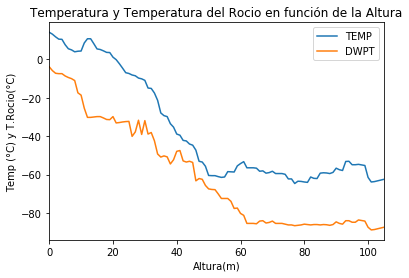
\includegraphics[width=0.5\textwidth]{TemperaturasDic.png}
    \centering
    \label{TEMPS}
\end{figure}
\begin{figure}[H]
    \caption{Temperatura y Temperatura del Roció (Junio)}
    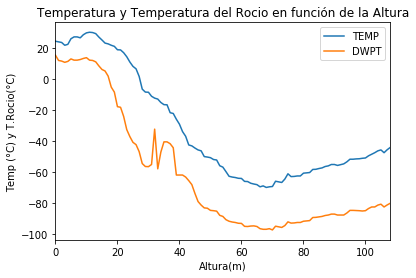
\includegraphics[width=0.5\textwidth]{TemperaturasJun.png}
    \centering
    \label{TEMPS}
\end{figure}
En estas gráficas se nota una diferencia para ambas variables. La temperatura del roció baja considerablemente rápido en el mes de diciembre, y se mantiene baja para el final de este, mientras que en el mes de junio baja para luego elevarse un poco al final del mes. Sucede algo similar con la temperatura en ambos meses. Si bien el comportamiento es el mismo, los datos tienen una variación considerable.

Las siguientes gráficas son de las velocidades del viento en nudos para ambos meses.
\begin{figure}[H]
    \caption{Rapidez del viento (Diciembre)}
    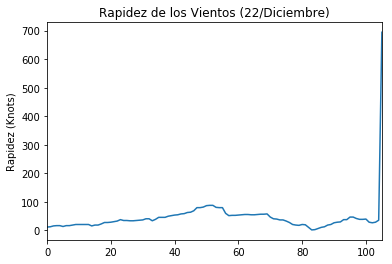
\includegraphics[width=0.5\textwidth]{RapidezVientoDic.png}
    \centering
    \label{VIEN}
\end{figure}
\begin{figure}[H]
    \caption{Rapidez del viento (Junio)}
    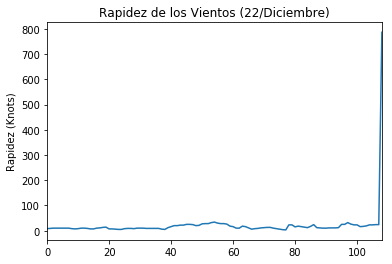
\includegraphics[width=0.5\textwidth]{RapidezVientoJun.png}
    \centering
    \label{VIEN}
\end{figure}
Estas gráficas también muestran un comportamiento similar, no obstante, se observa que en el mes de diciembre la velocidad de los vientos fue mayor y un poco más variable que en el mes de junio. 

Por último, un par de gráficos de la humedad relativa en función de la altura
\begin{figure}[H]
    \caption{Variación de la Humedad Relativa (Diciembre)}
    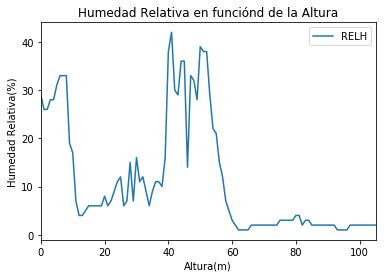
\includegraphics[width=0.5\textwidth]{HRDic.png}
    \centering
    \label{HUM}
\end{figure}
\begin{figure}[H]
    \caption{Variación de la Humedad Relativa (Junio)}
    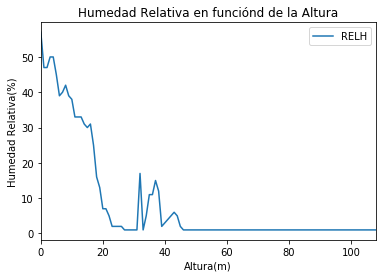
\includegraphics[width=0.5\textwidth]{HRJun.png}
    \centering
    \label{HUM}
\end{figure}
En estas dos gráficas se muestran comportamientos distintos para cada mes, mientras que en el mes de junio la humedad relativa empieza en un nivel alto, y empieza a decaer conforme cambio el tiempo, para el mes de diciembre, se tiene un comportamiento más "errático", donde la humedad relativa sube y baja.

\section{Conclusiones}
Después de analizar con cuidado los gráficos obtenidos, llegue a la conclusión de que los fenómenos meteorológicos no son ni de cerca constantes, que estos varían mucho de un mes a otro, e incluso pueden variar demasiado de un día a otro.

\section{Bibliografía}

\section{Ápendice}

\begin{enumerate}
\item ¿Cuál es tu opinión general de esta actividad?
Creo que es una actividad interesante para el reforzar la introducción al entorno de Jupyter Notebook, así como para la práctica de la creación de gráficas, o manejo de datos.

\item ¿Qué fue lo que más te agrado?, ¿Qué fue lo que menos te agrado?
Me agrado el hecho de que era bastante parecida a la práctica anterior, de modo que no me sentí muy perdida al trabajar en ella, ya que tenía un conocimiento provió de como hacer las cosas.

\item ¿Qué consideras que aprendiste en esta actividad?
Aprendí a manejar con más sencillez la creación de gráficos, y empecé a entender mejor la manera de trabajar en Jupyter Notebook.

\item ¿Qué le falto?, ¿Qué le sobro?
No considero que haya faltado o sobrado algo.

\item ¿Qué mejoras sugieres a la actividad?
Quizás, añadir un ejemplo sobre como hacer limites en el rango de los datos.

\end{enumerate}



\end{document}
